%
% File acl2012.tex
%
% Contact: Maggie Li (cswjli@comp.polyu.edu.hk), Michael White (mwhite@ling.osu.edu)
%%
%% Based on the style files for ACL2008 by Joakim Nivre and Noah Smith
%% and that of ACL2010 by Jing-Shin Chang and Philipp Koehn


\documentclass[12pt]{article}
\usepackage{poneil_jhong}
\usepackage{times}
\usepackage{latexsym}
\usepackage{amsmath}
\usepackage{multirow}
\usepackage{url}
\usepackage{graphicx}
\DeclareMathOperator*{\argmax}{arg\,max}
\setlength\titlebox{6.5cm}    % Expanding the titlebox

\title{Meta Dynamic Programming}

\author{Juneki Hong \\
  Johns Hopkins University \\
  {\tt juneki@jhu.edu} \\\And
  Paul O'Neil \\
  Johns Hopkins University \\
  {\tt poneil1@jhu.edu} \\}

\date{}

\begin{document}
\maketitle
\begin{abstract}
  We built a server in order to perform multiple exact local alignment problems. This server manages a storage database and worker nodes in order to handle queries made by clients. As clients send many local alignment problem requests, we want to be able to store and cache previous solutions for use later. The client-server architecture will provide a framework for this task. We discover that the biggest issues that our approach faces is network latency and the overhead of our message passing protocols. 
\end{abstract}


\section{Introduction}
%Why work on this? Why your approach?
The task of local alignment is a frequently queried task in Computational Genomics. 
An individual local alignment problem can be solved by computing a matrix of values using Dynamic Programming, but what if parts of a problem matrix could be reused in future alignment tasks? We want to use previous Dynamic Programming problems to help solve future problems. In other words, we want to perform Dynamic Programming across Dynamic Programming problems: Meta Dynamic Programming.

When many queries for local alignment are made, there might be similar structure across tasks that could be reused. For example, when aligning gene sequences, similar subsequences could reappear because they were all taken from similar organisms, there were repeating genes in certain sections of genomes, or even simply by chance because of the limited permutations of the gene alphabet A,C,G,T.

We chose to build a server in order to receive alignment requests, store past queries, and then return the result. This server can serve as a central location for previous alignment tasks, where we could try to fetch a solution from a database, or solve the problem when none were available. With this server in place, it could be possible to explore different ways we can exploit the similarities across our problems.
 



\section{Prior Work}
% What did you read? What did others accomplish before you?

Previous approaches to faster local alignment exist in the form of performing Smith-Waterman with SIMD parallelization \cite{Rognes:11}. This approach solves a given problem matrix in its entirety. However, they gain a large speed boost by arranging the problems to be better exploited by the CPU or CUDA. 

Another approach to fast local alignment is Z-align\cite{Rognes:11}. In this scheme, local alignment problems are broken up and allocated across multiple processors, and message passing between the processors helps compute the solution.

Z-align would be closer to our approach, where we want to break up a problem and perform message passing to find a solution. However, we want to provide a server working across a network instead of being confined to one machine.  

We want to additionally store previous results and try and identify sections of the matrix that we don't have to do in the first place, while working on solving the rest. It might be possible to do a combination of our approach with the above methods, in that when it comes time to completely solve a problem, we would want to do it quickly.

\begin{figure}
  \centering 
  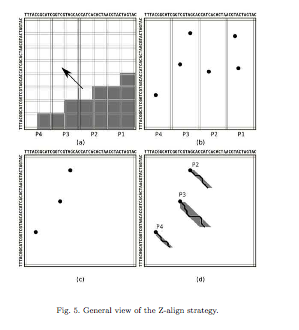
\includegraphics[width=0.5\textwidth]{ExistingWorkAllocationStrategies}
  \caption{Illustration of Z-align.\cite{Rognes:11}}
  \label{fig:z-align}
\end{figure}



\section{Methods and software}
%What did you implement? Why? How?

%TODO cite msgpack and boost.
Our server was implemented in C++ with the help of the Msgpack library for data serialization, and the Boost library for socket IO and help parsing command line arguments. The implementation of the server is broken up into parts, described by our architecture.

\subsection{Problem Specification}
One of the main ideas behind our approach is that a local alignment problem can be described by four sequences and a number: The two genome sequences we are trying to align, two initial sequences of numbers representing the top row and left-most column of the matrix, and one number representing the top-left corner of the matrix (if applicable). This in effect uniquely ``identifies'' a problem, and every problem with these four matching sequences and corner will have the same solution. The architecture of our project is designed around passing around and storing these problem specifications to complete the task.


\subsection{Architecture}
Our project divides into four sections: A Client, a Leader, Storage, and Workers. This allows for us to better modularize the tasks performed by a local alignment server, and it gives abstractions and interfaces for the components to call. For example, it does not matter to the Leader and Worker classes what the real backing implementation of Storage is, as long as the store and query calls work. This framework is what will allow us to change or upgrade components in the future. 

This architecture also allows us to have many worker nodes being managed by a Leader, increasing our problem solving capacity. 
We could also potentially have multiple Leader nodes and Storage nodes as well, especially if our system were to scale up to handle much larger requests.

\subsubsection{Client}
The Client uploads genomes to the Leader, and then sends queries for local alignment problems. The Leader pass on uploaded genomes to Storage, and then handle the alignment queries by responding with solutions. The solutions returned will be a completed matrix and the location of the maximum value.

\subsubsection{Leader}
The Leader handles queries from the Client as well as allocates work to Workers and manage the solutions. A Leader can allocate work to a Worker by specifying the border initialization, both of the genome sequences and the first numerical row and column to fill out the rest of the matrix. A Worker can complete a solution and inform the Leader of its location in Storage. Once a solution has been indicated, a Leader can then query Storage to pick it up, to send back to the Client. 

\subsubsection{Storage}
The Storage is a database for the Leader and Worker to store and query items such as genomes, and solutions to alignment problems. Genomes have identifications that can be matched against, and alignment problem solutions matched by their problem description. 
A Worker will produce solutions and store them into Storage. It will also check to see if a solution already exists, and if so it does not have to do any additional work.

\subsubsection{Worker}
When a Worker is ready, it queries the Leader asking for problems to work on. The Leader can then respond with problems that can be claimed. A Worker then claims a problem specification, checks storage, and if applicable, fills out the solution and sends it off to Storage. It responds to the Leader that it is finished.



\begin{figure}
  \centering 
  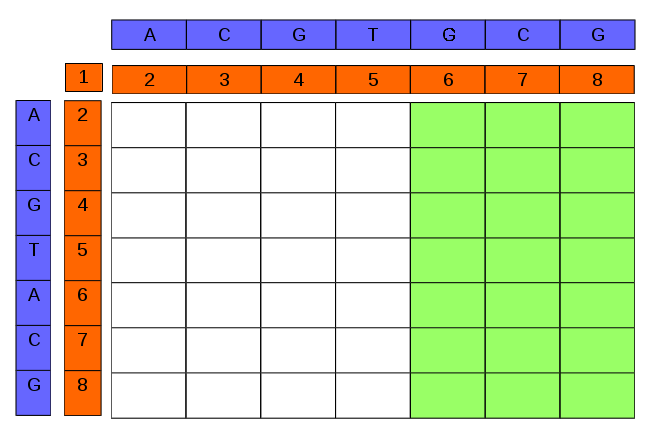
\includegraphics[width=0.5\textwidth]{problem2}
  \caption{What a problem for local alignment looks like. A problem description includes two genome sequences, numerical row and column initializations, and a corner number}
  \label{fig:problem}
\end{figure}




\subsection{Improvements, Speedups}
After a base system of this architecture was implemented, there were some several improvements that were made. Some notable ones include:

\subsubsection{Available Workers Put on Hold}
When a Worker requests for a list of problems, the Leader does not immediately close the connection if there are none, but instead keeps a list of available Workers that it can broadcast to when new problems are available. This cuts down some of the network overhead when a Worker is ready for new problems. 

\subsubsection{Workers Randomly Select Problems}
The Worker also now select randomly from the list of problems instead of just the first one. If multiple Workers were contacting the Leader, they would have both tried to claim the same problems, and so this behavior has been alleviated to a degree. In order to cut down on the network overhead even further, the Worker also tries to claim multiple problems at once, and then solves them returning the results one at a time.

\subsubsection{Storage send out ACKs Immediately}
Finally, when uploads to Storage are being made, we changed the protocol such that Storage would send the acknowledgement first before it had finished serializing the received data. Although this might be vulnerable from an systems perspective, where the storage could fail while it is receiving data, we wanted to diminish the amount of time the Worker and Leader has to wait for a response while Storage receives data.


\subsection{Features Not Completed}
There were some features that we attempted or wanted to put into the system that did not work out because of its complexity or because of implementation issues. Some notable ones include:

\subsubsection{Problem Subdivision}
A feature we wanted the Leader to have was problem subdivision, where the Leader would break down the task of completing a matrix into subproblems of smaller matrices, and then later reassemble the full solution from the pieces. The Leader would then have to keep track of which original problems that the subproblems belonged to, when the subproblems completed the full problem, and then reassemble the solution matrices.
  
When we implemented this feature, we introduced bugs that interfered with the operation of the Leader and Storage, so we had to remove it. The Leader currently sends entire problem specifications to the Workers instead of problem chunks to be reassembled later. This means that the cache hits will only consist of exact matches of local alignment problems we have seen earlier. 


\begin{figure}
  \centering 
  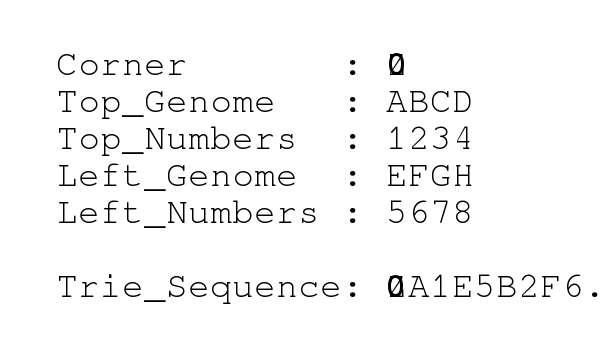
\includegraphics[width=0.5\textwidth]{trie_corrected}
  \caption{An example Trie Sequence for partial or approximate matching, with the four sequences and corner number given.}
  \label{fig:trie}
\end{figure}


\subsubsection{Partial Solution Matching}

Another feature we wanted Storage to have was partial solution matching. Given a problem specification, a Worker will query into Storage checking to see if it already exists, and it might be possible for Storage to return a solution that mostly matches what the Worker was looking for. This would allow the Worker to fill in most of their matrix easily, fill in the rest manually, and then return the solution.

We will accomplish this with a type of Trie data structure, traversing down the Trie with a problem specification by alternating and matching each of the four sequences. For example, we would traverse the Trie by matching the corner, then the first character of the first genome, the first number of the top row, the first character of the second genome, the first number of the first column, then the second character of the first genome, etc. 

In this way, the Trie is matching the upper left corner of a problem and progressively growing out, and traversing further down the trie represents a better partial solution match. See figure 3.




\subsection{Future Work}
In addition to building the protocols and networking of our base system, as well as trying to implement the above features, we also have additional ideas that constitute future work.

\subsubsection{Dynamic Problem Subdivision}
As a step further from Problem Subdivision, we would like to explore dynamic subdivision, where the Leader does not break down a task into regular sized chunks, but rather dynamically take subsections as large or small as it wanted, according to how likely it felt that the chunks would be useful in the future.

Some approaches to this could include training a language model for gene sequences, to find the probability of a sequence (up to a length k) in order to help us decide which subsequences are likely enough for us to see again in the future.

Another approach could be to exploit genome meta-data. If we were about to see many human sequence reads instead of E. Coli, this might influence our decision-making process.

% TODO: Paul
%Another idea could be to preprocess the alignment problem, computing only down the diagonal and filling the other areas of the matrix with zeros, in order to see where the genomes are similar to each other.



\subsubsection{Worker-Side Cache}

Another feature we are considering is allowing the Workers to cache some of their own solutions. When a Worker claims a problem to work on, it can first check its own cache to look for an exact or partial match, instead of just going to Storage. It can then fill out the solution quickly and respond back to the Leader without ever having gone to Storage. 

A Worker can also use its cache to be smarter about which problems it claims. By comparing a problem list to its cache, a Worker could claim problems it already knows solutions to. If it implements its own Trie, it could do partial matching as well.

These approaches will help reduce network latency, and possibly help the Workers self-specialize.






\section{Results}
%How well did your method work compared to others?

We ran our experiments with genome data found in the PREFAB database \cite{Edgar:04}.

We loaded in X many sequences and aligned them all with each other producing X alignment requests. We ran our server with several different configurations against a baseline of a C++ program that would naively solve every alignment problem filling out the matrix. We wanted to compare the relative performance of our server with storage caching turned on and off, how increasing the number of workers would impact performance, and how all of that compared to the baseline system.

\begin{figure*}
  \centering 
  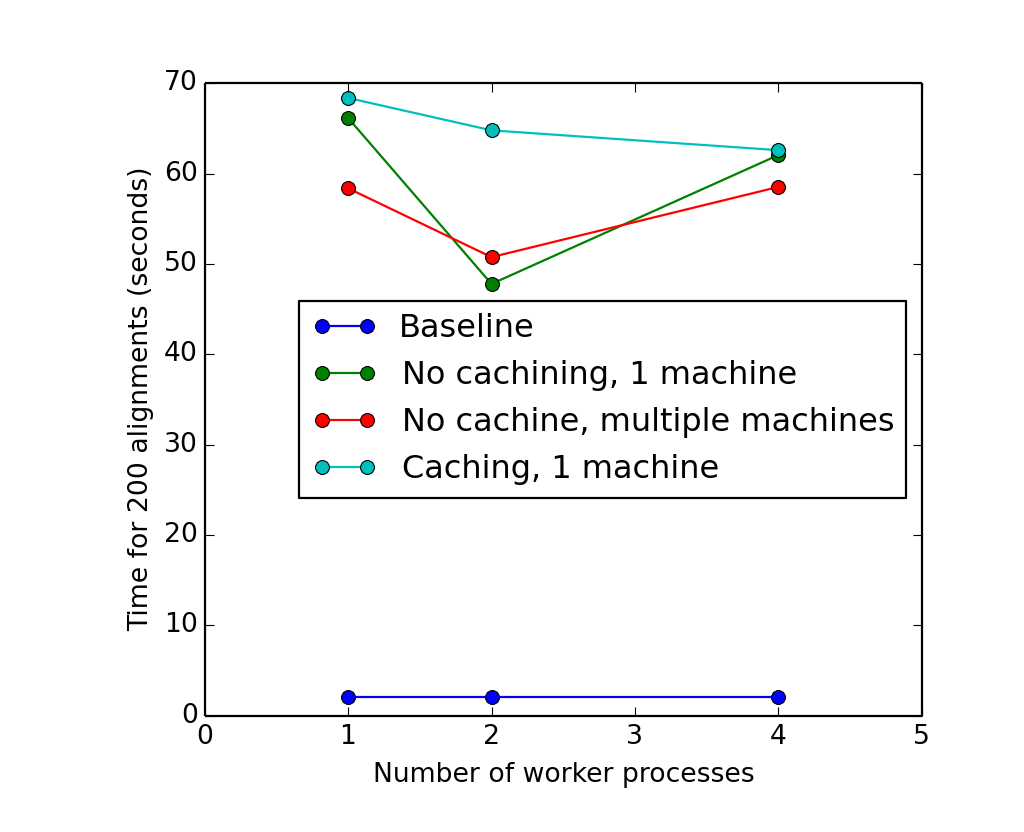
\includegraphics[width=0.7\textwidth]{benchmarks}
  \caption{Our benchmarks all on one plot.}
  \label{fig:benchmarks}
\end{figure*}



\section{Conclusions} 
%What did you learn? What should we come away with?

The overwhelming issue for our alignment server was the network overhead within the architecture. Even with a variety of different server configurations, the overall performance turned out to be similar because the vast majority of time was spent on network calls. 

For a complete version of our server, we would need to optimize these network calls as much as possible. For example, we could try and reduce or limit the amount of acknowledgment replies that are required by our protocol, as well as find ways to ``batch'' calls, commands, and requests all together.

We will also need to do further testing on different and much bigger problem sizes, to see how that fares among our trials. If the size of the problems became large enough to become comparable to the network latency, then we might be able to beat the naive baseline with the amount of parallelism we could afford among all of the Worker nodes.

The baseline naive program outperformed our system by about a factor of 20.


\section{Works Cited}





\begin{thebibliography}{}

\bibitem[\protect\citename{Boukerche}2012]{Boukerche:12}
Azzedine Boukerche.
\newblock 2012.
\newblock {\em Exact Parallel Alignment of Megabase genomic Sequences with Tunable Work Distribution},
\newblock International Journal of Foundations of Computer Science 23(2), 407-429.

\bibitem[\protect\citename{Rognes}2011]{Rognes:11}
Rognes, Torbj.
\newblock 2011.
\newblock {\em Faster Smith-Waterman Database Searches with Inter-sequence SIMD Parallelisation}
\newblock BMC bioinformatics 12(1), 221.

\bibitem[\protect\citename{Edgar}2004]{Edgar:04}
Edgar, Robert C.
\newblock 2004.
\newblock {\em MUSCLE: multiple sequence alignment with high accuracy and high throughput}
\newblock Nucleic Acids Research 32(5), 1792-97.





%\bibitem[\protect\citename{Aho and Ullman}1972]{Aho:72}
%Alfred~V. Aho and Jeffrey~D. Ullman.
%\newblock 1972.
%\newblock {\em The Theory of Parsing, Translation and Compiling}, volume~1.
%\newblock Prentice-{Hall}, Englewood Cliffs, NJ.

%\bibitem[\protect\citename{{American Psychological Association}}1983]{APA:83}
%{American Psychological Association}.
%\newblock 1983.
%\newblock {\em Publications Manual}.
%\newblock American Psychological Association, Washington, DC.

%\bibitem[\protect\citename{{Association for Computing Machinery}}1983]{ACM:83}
%{Association for Computing Machinery}.
%\newblock 1983.
%\newblock {\em Computing Reviews}, 24(11):503--512.

%\bibitem[\protect\citename{Chandra \bgroup et al.\egroup }1981]{Chandra:81}
%Ashok~K. Chandra, Dexter~C. Kozen, and Larry~J. Stockmeyer.
%\newblock 1981.
%\newblock Alternation.
%\newblock {\em Journal of the Association for Computing Machinery},
%  28(1):114--133.

%\bibitem[\protect\citename{Gusfield}1997]{Gusfield:97}
%Dan Gusfield.
%\newblock 1997.
%\newblock {\em Algorithms on Strings, Trees and Sequences}.
%\newblock Cambridge University Press, Cambridge, UK.

\end{thebibliography}

\end{document}
